\chapter{Attack Evaluation}
\label{chap:analysis_and_results}

In this chapter we provide an in-depth evaluation of the attack. Our main stream experiment is based on one smartwatch-phone pair: \textit{Huawei-Pixel}. Tab.~\ref{tab:main_watch_spec} shows the specifications of these two devices. In the first part of this chapter we analyze the results we get on this smartwatch-phone pair. After that, we see if the results also apply to two different pairs of devises (\textit{Fossil-Nexus} and \textit{AppleWatch-iPhone}). We finally summarize the results in the last Section.
\\

\begin{table}[ht]
    \caption{Specification of the main stream experiment's smartwatch-phone pair.}
    \label{tab:main_watch_spec}
\centering
\subcaption*{ \textbf{Huawei   -    Pixel}}
 \begin{tabular}{@{}lll@{}} 
 \toprule
  & smartwatch & phone \\ [0.5ex] 
 \midrule
 Manufacturer & Huawei & Google \\ 

 Model & Huawei watch 2 (LEO-BX9) & Pixel 2  \\

 OS version & wearOS 2.16 & Android v9  \\
 \bottomrule
\end{tabular}

\end{table}



\section{Application Opening Identification}
\label{sec:application opening identification}
We will first focus on simply targeting \texttt{open} action, i.e. fingerprint traces when we simply open one particular application. We believe that targeting this kind of action has two benefits: First, this is the simplest action and does not require any encoding in our automation system. But most importantly, opening is not influenced by a specific user pattern interaction with the smartwatch and would be the best candidate for successful fingerprinting in the wild.


\subsection{Filtering out Applications} 
\label{subsec:Filtering out Application}
Before starting our analysis, we suspect some applications to not send any data at opening. Which seems to be a realistic supposition as many applications should be self-sufficient at startup. To verify this, we ranked classes (i.e, opening action for different applications) according to the median of their total amount of data transfer against their accuracy. Fig.~\ref{fig:acc_ranked} shows the difference between ordering accuracy by class index (see Tab.~\ref{tab:initial_Apps}) and by data transfer size. From the right plot, we can clearly distinguish two clusters. The bottom left cluster contains applications that did not send data at opening, or at least not enough. Indeed, we can still see classes belonging to the bottom left cluster sending 212 bytes at the median. This could be due to background data communication such as push notification or background updates, or it could be that the amount of data sent by this application is not sufficient to classify it reliably. We notice that some applications have pretty high accuracy in this same cluster. This is explained by the fact that since they are only misclassified amongst themselves the random correct guess is more likely. Also, the classifier might have learnt a persistent background noise across different instances of the same class.
\\

\begin{figure}[H]
\centering
\begin{subfigure}{.5\textwidth}
  \centering
  \includegraphics[width=1\linewidth]{figures/plots/scatter_plot_accuracy_size_unordered.png}
\end{subfigure}%
\begin{subfigure}{.5\textwidth}
  \centering
  \includegraphics[width=1\linewidth]{figures/plots/scatter_plot_accuracy_size_ordered.png}
\end{subfigure}
\caption{\textbf{Left:} Classes accuracy ranked by class index. \textbf{Right:} Classes accuracy ranked by data transfer size median.}
\label{fig:acc_ranked}
\end{figure}


We filter out the of none-communicating application with the following formula:

$$ out = \{a:Pr(a_s<200) > 0.25\} $$

Where $a_s$  is the total amount of data (in bytes) captured when application $a$ is launched.
\\

Put into words, we filter out applications for which the amount of data captured when launched is less than 200 bytes more than 25\% of the time. We choose 200 because it seems to be the last value on the x-axis belonging to the first cluster (212 on Fig.~\ref{fig:acc_ranked}'s realisation). In fact, the fist class belonging to the second cluster has a median of 603, far beyond 200. 0.25 is chosen because we reckon that if the application really does not communicate, an intense background noise would not be present in more than 25\% of the captures.
\\ 

This particular filter removed 17 applications out of 55 in our dataset\footnote{The list of application indexes that does not communicate in out experiment are the following: \{1, 2, 4, 5, 12, 14, 21, 24, 25, 26, 32, 36, 37, 40, 45, 53, 55\} (see Tab.~\ref{tab:initial_Apps})}. We note that for two filtered applications (GooglePay and ASB mobile banking), we were unable to create user account\footnote{GooglePay because it required a password which might have influenced our experiment and ADB because it required an housing in New-Zeland, which unfortunately we do not have.}, which might affect the way the app normally communicate with the phone. Moreover, these applications are filtered only based on opening. This does not mean that another action does not trigger the communication enough to be fingerprinted, as we will see in Sec.~\ref{sec:in-App}. 
\\

By analogy to Fig. \ref{fig:app proportio}, we show the effect of filtering on the selected applications in Fig. \ref{fig:app proportion filtered}. We see that the type of applications affected the most by the filtering is the religious-related apps. Indeed, out of the four selected religious applications, two where simply offline excerpt of religious text. In contrast, the news, map and messaging application need to collect online resources and are not affected by the filtering.

\begin{figure}[h]
\centering
\begin{subfigure}{.5\textwidth}
 \centering
  \includegraphics[width=0.65\linewidth]{figures/plots/Apps criteria repartition filtered.png}
  \label{fig:sub1}
\end{subfigure}%
\begin{subfigure}{.5\textwidth}
  \centering
  \includegraphics[width=0.95\linewidth]{figures/plots/Apps typle repartition filtered.png}
  \label{fig:sub2}
\end{subfigure}
\caption{\textbf{Left:} Proportion of filtered applications by criteria. \textbf{Right:} Proportion of filtered applications by types}
\label{fig:app proportion filtered}
\end{figure}



\newpage

\subsection{Results on Apps Opening} After removing application that does not communicate at opening, we are left with 38 applications. We performed cross validation with 50 random splits on 38 samples per application, and got an averaged accuracy over all predictions of \textbf{96.8\% (+/- 2\%)}\footnote{We use this notation to denote the 95\% confidence interval.}. A realisation of a classification on this experiment is shown in Fig.\ref{fig:cm_open_huawei}. From the confusion matrix, we see that 31 apps have perfect accuracy score and the lowest accuracy score is 80\% (Fit, Qardio and Workout). 

\begin{figure}[H]
 \centering
 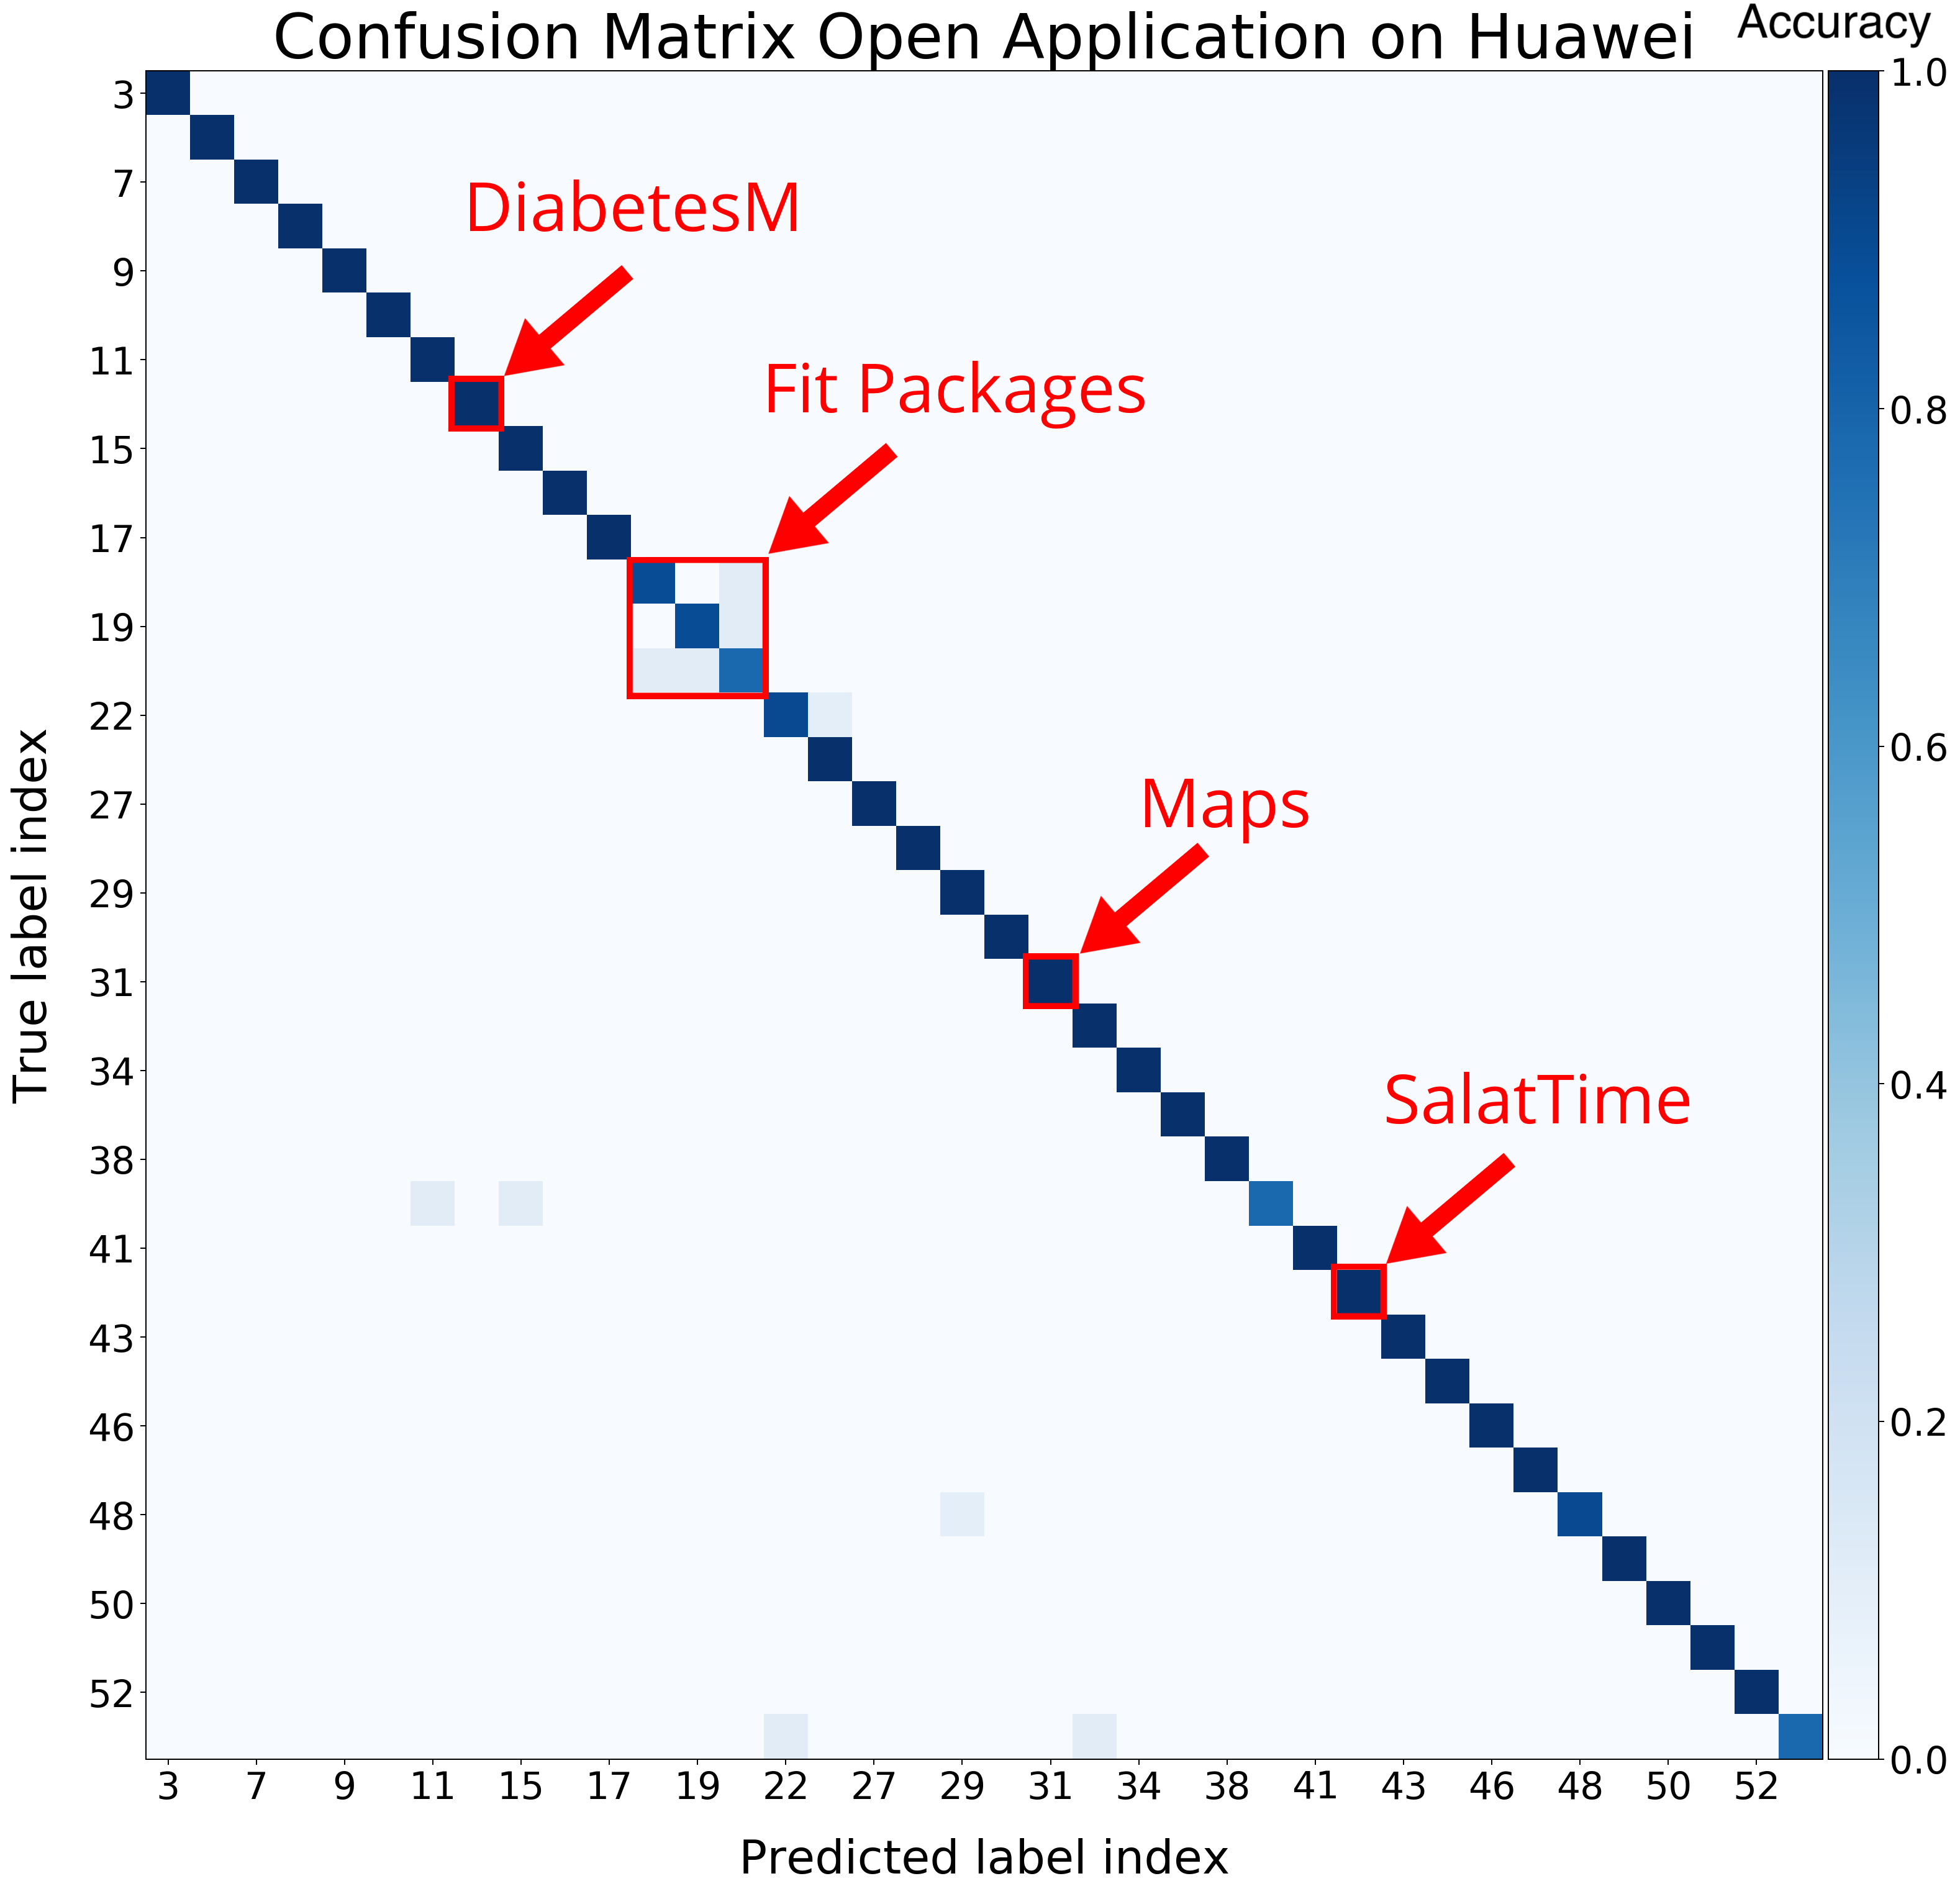
\includegraphics[width=0.70\textwidth]{figures/cm/Confusion_matrix_for_huawei_annoted.png}
 \caption{Confusion Matrix for open action on Huawei smartwatch.}
  \label{fig:cm_open_huawei}
\end{figure}


\newpage


\subsection{Number of Samples \label{data_set_size_per_class}
per Class vs Accuracy} Since generating data takes a long time, we investigate the impact of the number of samples per class on the accuracy to see how much accuracy an attacker might expect according to his dataset size. For this, we increasingly augmented the size of our dataset from n=2 to 30 samples per application. For each n, we picked 15 times n samples per class at random and performed 5 random split with 25\% test to extract the mean and the variance. We then average the mean and the variance over these 15 times. Fig.~\ref{fig:plot_accuray_dataset_size} plots the accuracy at different dataset size level.  We see that with a dataset size of 6 samples per class, we already achieve an accuracy of more than 90\% on average and with 11 samples per class more than 95\%. The variance also decreases. At 10 samples per class, we have less than 8\% accuracy lying inside the confidence interval, and at 24 samples per class, less than 4\%. 

\begin{figure}[ht]
 \centering
 \includegraphics[width=0.60\textwidth]{figures/plots/Accuracy_against_dataset_size_per_class_for_Huawei_final.png}
 \caption{accuracy against dataset size for 2 to 30 samples per application}
 \label{fig:plot_accuray_dataset_size}
\end{figure}






\section{In-App Action Identification}
\label{sec:in-App}
We saw in the previous Section that we can successfully identify applications at opening as long as it generates enough data. Now, we want to see at which point we can be precise in targeting specific actions within application. For instance, inside the application DiabetesM the user can perform several sensitive actions such as adding some glucose to his log book, or recording an insulin shot. Therefore, we launched the attack on a selected set of 17 specific in-app actions from six different applications (see  Tab.~\ref{tab:selected_actions}). We found out that over the 17 actions selected, the model has an accuracy of \textbf{68.2\% (+/- 7.1\%)}. Which is around 62\% more than the random guess. By looking at the confusion matrix in Fig.~\ref{fig:in-app huawei}, we see that actions within the same application are more subject to misclassification amongst themselves, which is still a good news for an attacker who plans to discover the installed application. Moreover, this does not apply for all applications. For instance, the application Lifesum has two actions (indices 70 and 71) and still achieve 100\% accuracy.


\begin{figure}[H]
 \centering
 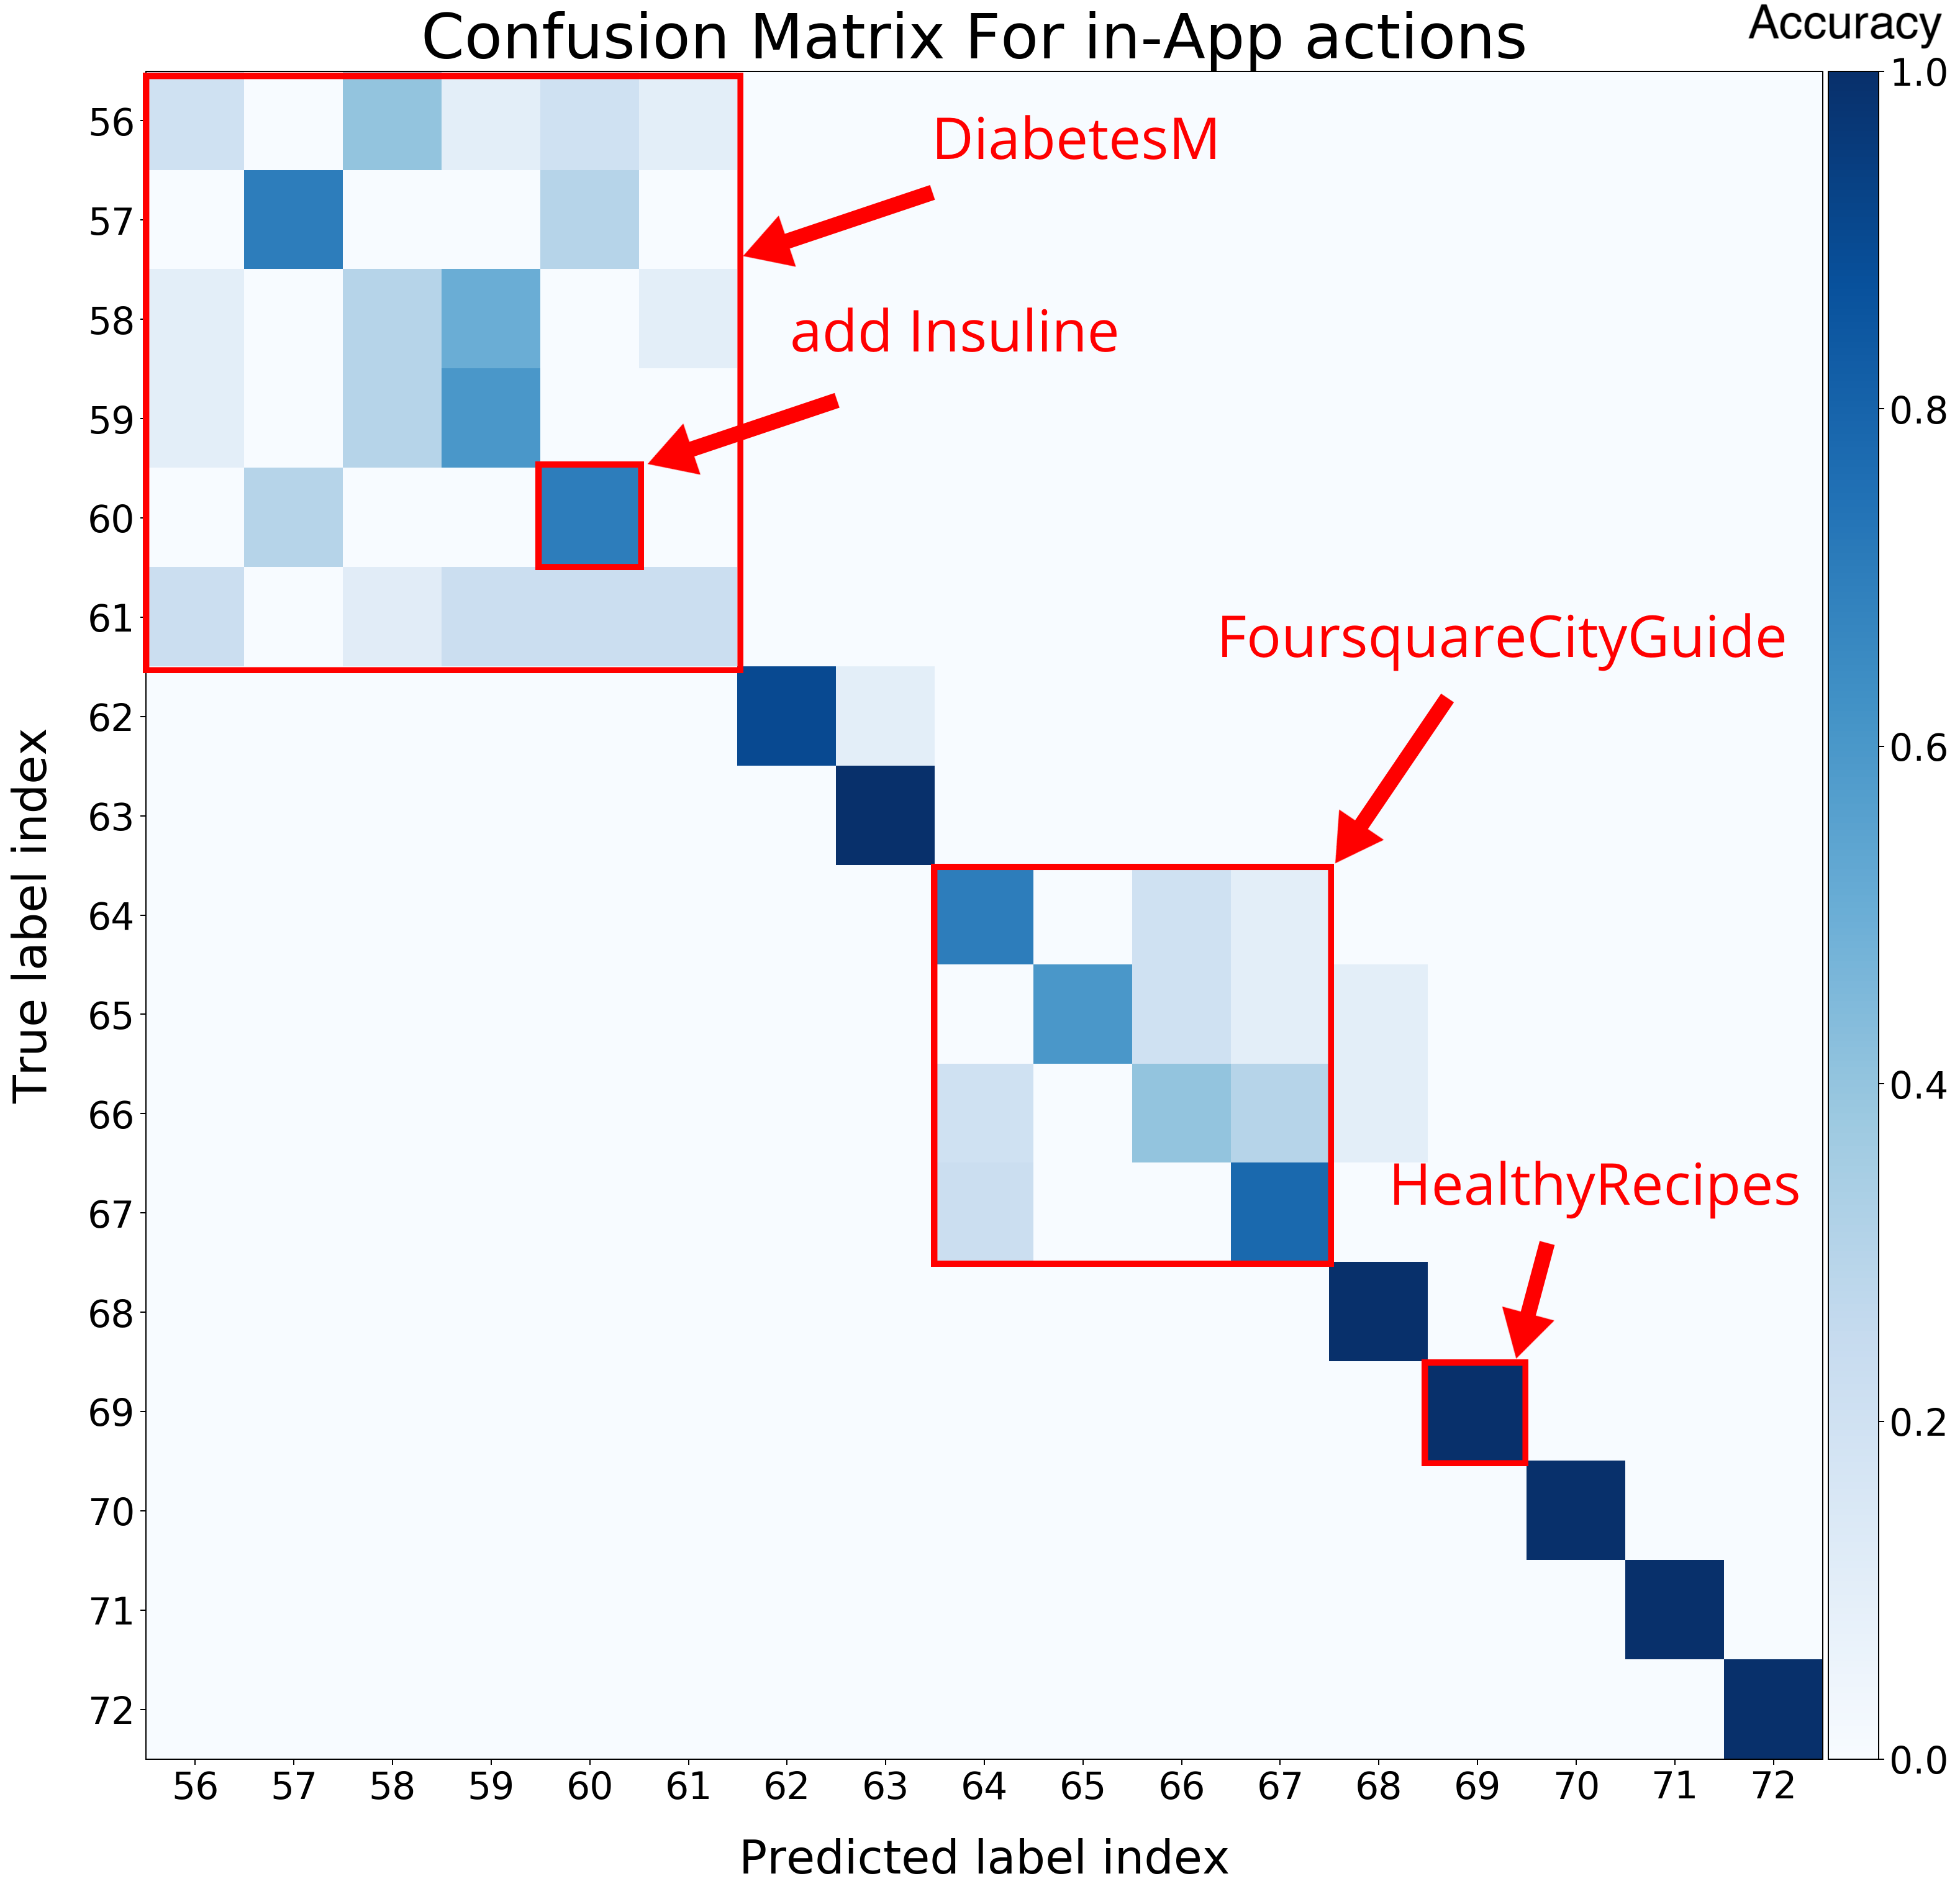
\includegraphics[width=0.7\textwidth]{figures/cm/all_inApp_action_annoted.png}
 \caption{Confusion matrix in-app actions on Huawei-Pixel.}
 \label{fig:in-app huawei}
\end{figure}


We note that the application HealthyRecipes was filtered out in Sec.~\ref{sec:application opening identification}. Even though at opening this app does not generate any traffic, we are still able to fingerprint it on a specific action (research Recipes in this case).









\section{Attack on Two Different Smartwatch-Phone Pairs}
We saw that the attack performs gracefully on one particular pair of devices. However, we want to show that the same attack also work on different smartwatch-phone pairs. Specifically, we selected two other smartwatch-phone pairs that differ in terms of Manufacturer, Model and OS version. Tab.~\ref{tab:extension_watch_spec} summarizes the specification of the two extra smartwatch-phone pairs. 
\\

\begin{table}[ht]
\begin{multicols}{2}
\centering
\subcaption*{\textbf{Fossil - Nexus}}
 \begin{tabular}{@{}lll@{}} 
 \toprule
  & watch & phone \\ [0.5ex] 
 \midrule
 Manufacturer & Fossil & LG Electronics \\ 

 Model & Q Explorist HR & Nexus 5  \\

 OS version & wearOS 2.16 & Android v6  \\
 \bottomrule
\end{tabular}
\subcaption*{\textbf{Apple Watch - iPhone}}
 \begin{tabular}{@{}lll@{}} 
 \toprule
  & watch & phone \\ [0.5ex] 
 \midrule
 Manufacturer & Apple & Apple \\ 

 Model & Apple Watch 5 & iPhone 8  \\

 OS version & watchOS 6.1.3 & iOS 13.3.1  \\
 \bottomrule
\end{tabular}

\end{multicols}
\caption{Specification of the smartwatch-phone pairs for the extended experiment.}
\label{tab:extension_watch_spec}
\end{table}


\paragraph{\textbf{Fossil - Nexus}.} For this experiment, we downloaded 35 applications out of the 38 applications tested on Huawei-Pixel (three of them were not compatible with the Fossil-Nexus pair\footnote{The three applications not compatible with the \textbf{Fossil - Nexus} pair are: \{3, 8,, 51\}, i.e. \{AppInTheAir, Camera, UARecord\}} at the time of the experiment). We collected 28 samples, performed 50 random splits with cross-validation and obtained an accuracy of \textbf{90.5\% (+/- 3\%)}. By looking at the confusion matrix in Fig.~\ref{fig:cm_fossil} we realize that the classes that are most misclassified are from the same native packages (Fit Package), this shows that these applications are very similar and reflects the possible difficulty to fingerprint actions belonging to the same application from Sec.~\ref{sec:in-App}. 


\begin{figure}[ht]
 \centering
 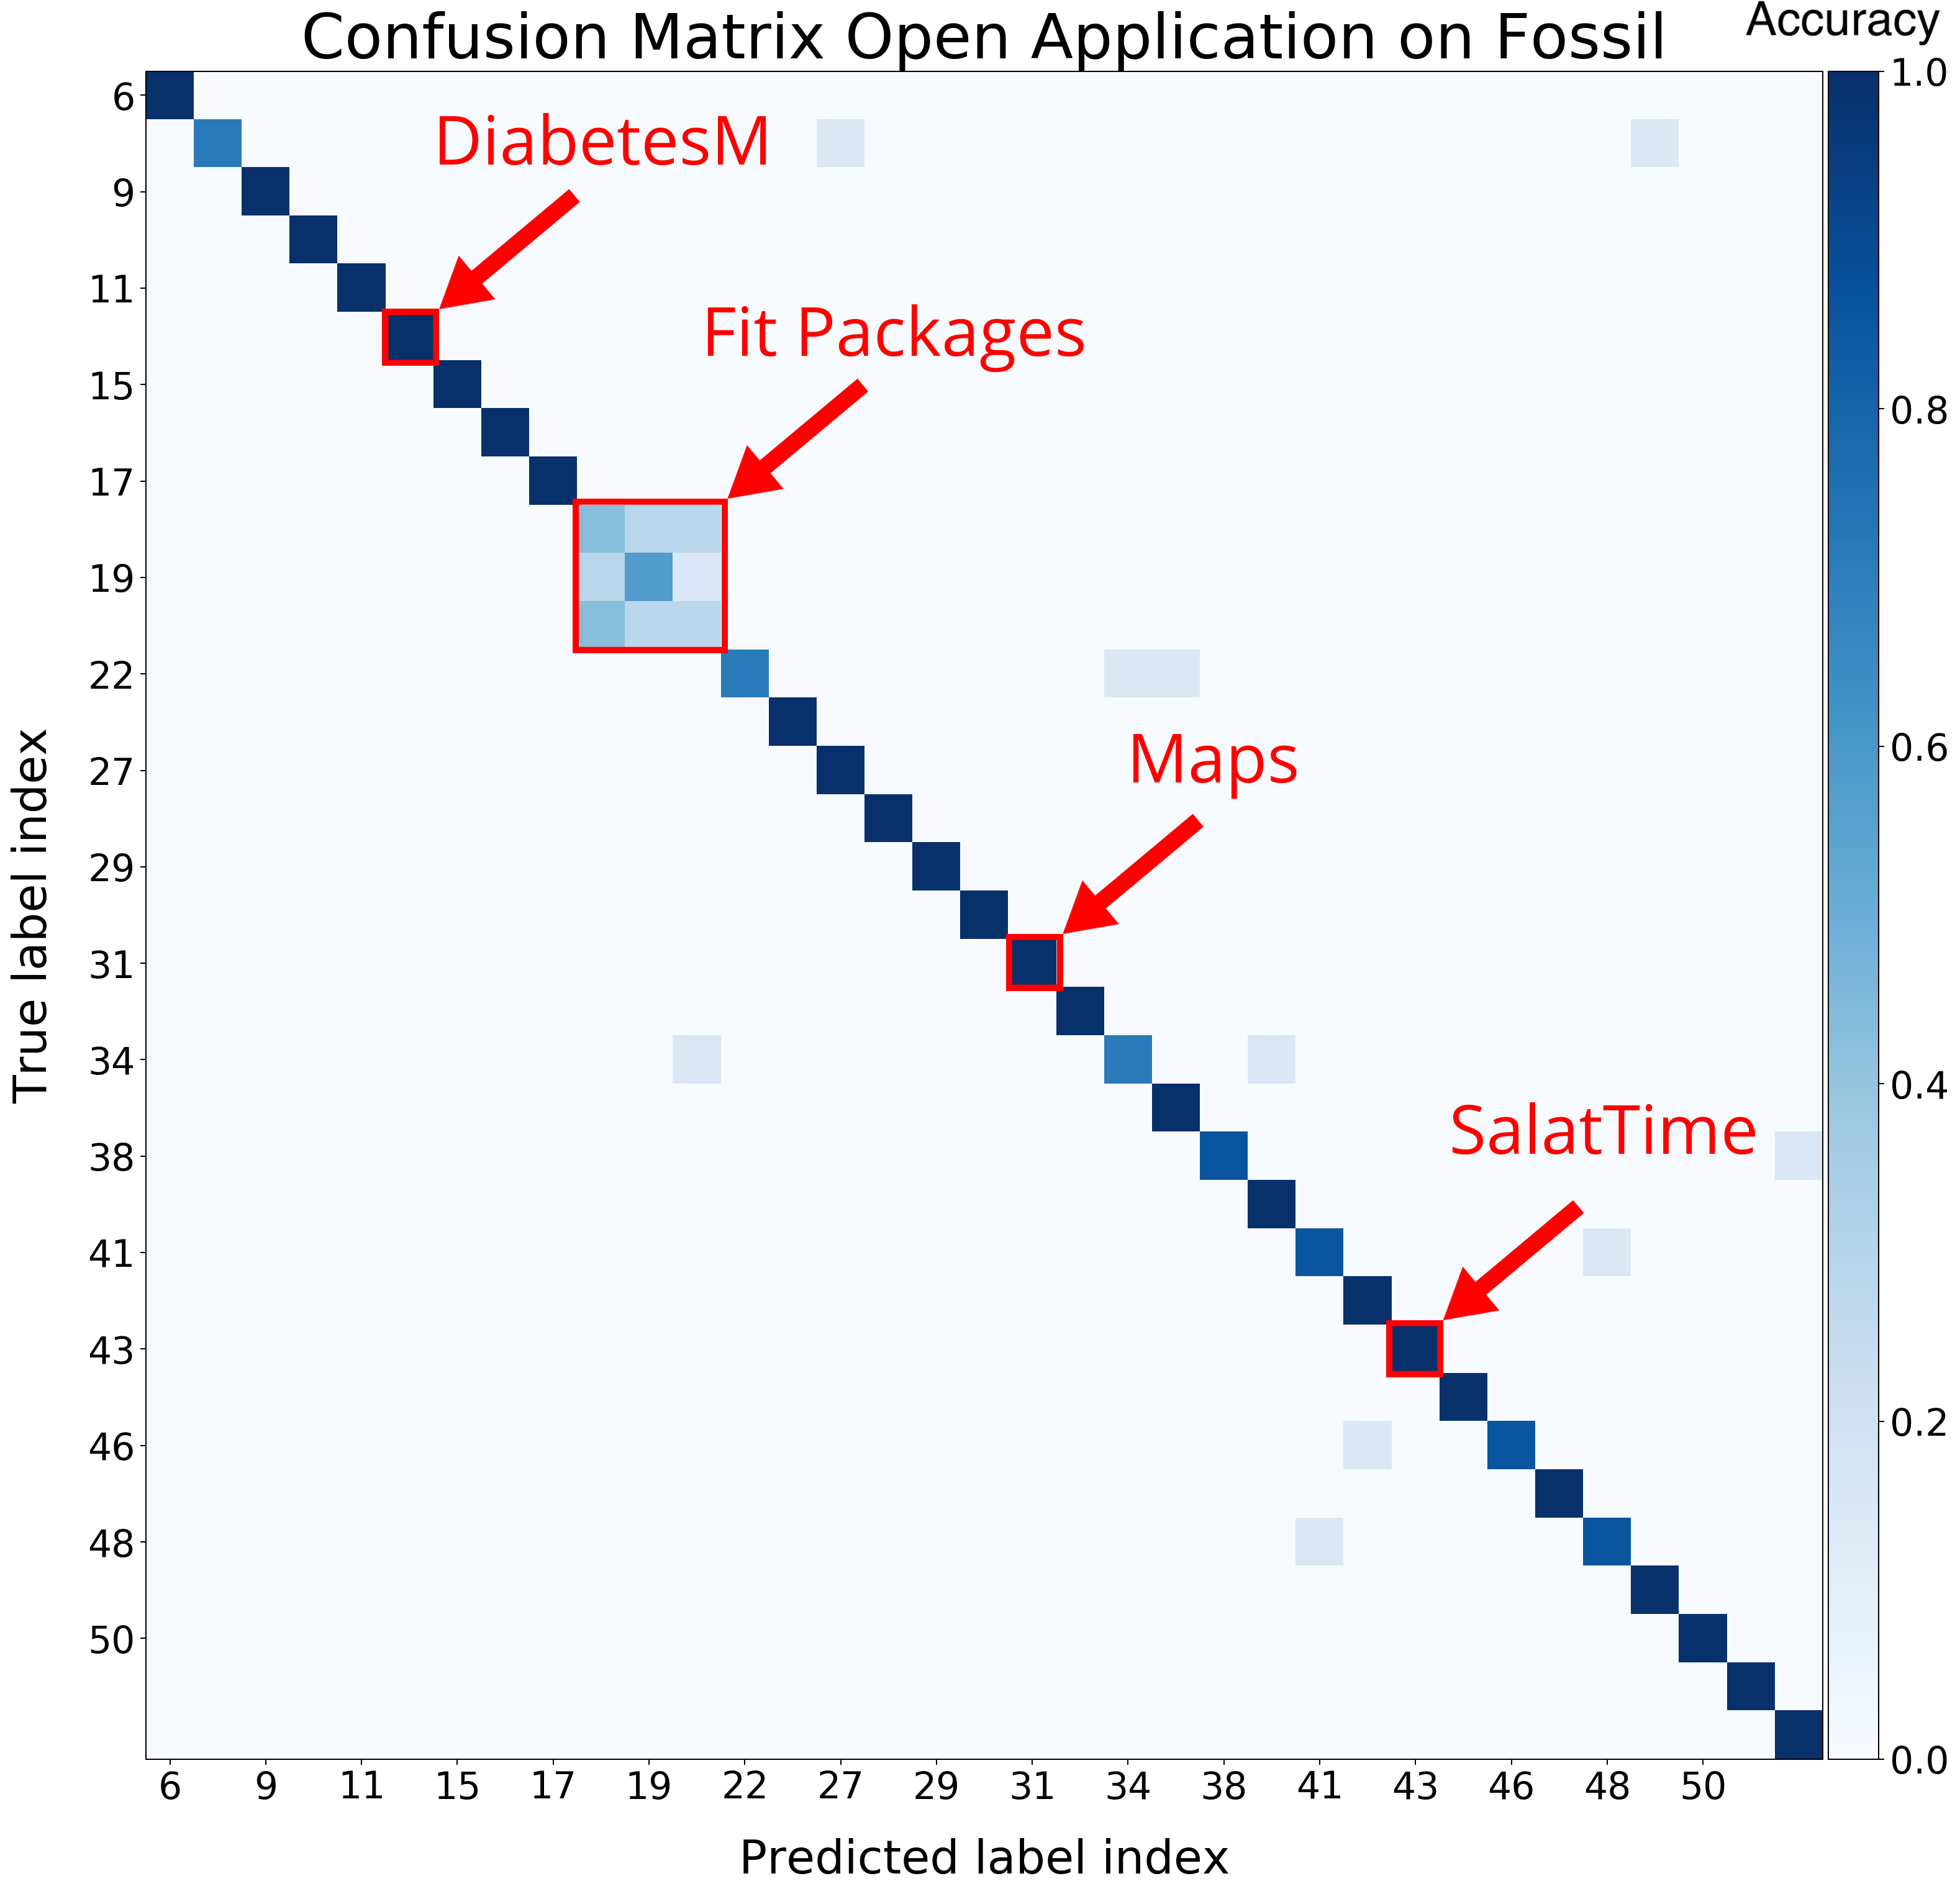
\includegraphics[width=0.70\textwidth]{figures/cm/Confusion_matrix_for_fossill_annoted.png}
 
 \caption{Confusion Matrix for open apps on Fossil smartwatch.}
 \label{fig:cm_fossil}
\end{figure}


\paragraph{\textbf{AppleWatch - iPhone.}}

We denote some differences between the AppleWatch - iPhone pair and the two previous pair of devices. First, the AppleWatch can transmit data over both Bluetooth Classic and Bluetooth LE requiring the attacker to possess a dual mode Bluetooth sniffer. Moreover, the connection is not persistent over Bluetooth Classic as it is on WearOS devices. This increases the difficulty to track the traffic. We also note that data transfer requiring low bandwidth tends to use BLE (apps such as PillReminder) in contrary, data transfer that requires higher bandwidth tends to use Bluetooth Classic (such as synchronizing electrocardiogram's data). In addition, as explained in Sec.~\ref{sec:data_generation}, we cannot automate the data generation and forces us to perform capture manually.  However, we show that even though these mechanisms seem to prevent an attack, we are still able to fingerprint the traffic with a good accuracy. Following the same guideline to evaluate the attack, we reach an accuracy of \textbf{88.7\% (+/- 7.5\%)} over 17 applications and 20 samples per application. The confusion matrix is shown in Fig.~\ref{fig:cm_iwatch}. We see that the lowest accuracy score is 40\% (20min.ch application). Out of the 17 applications tested, nine achieve perfect accuracy, such as ECG synchronization and RamadanTime.  




\begin{figure}[H]
 \centering
 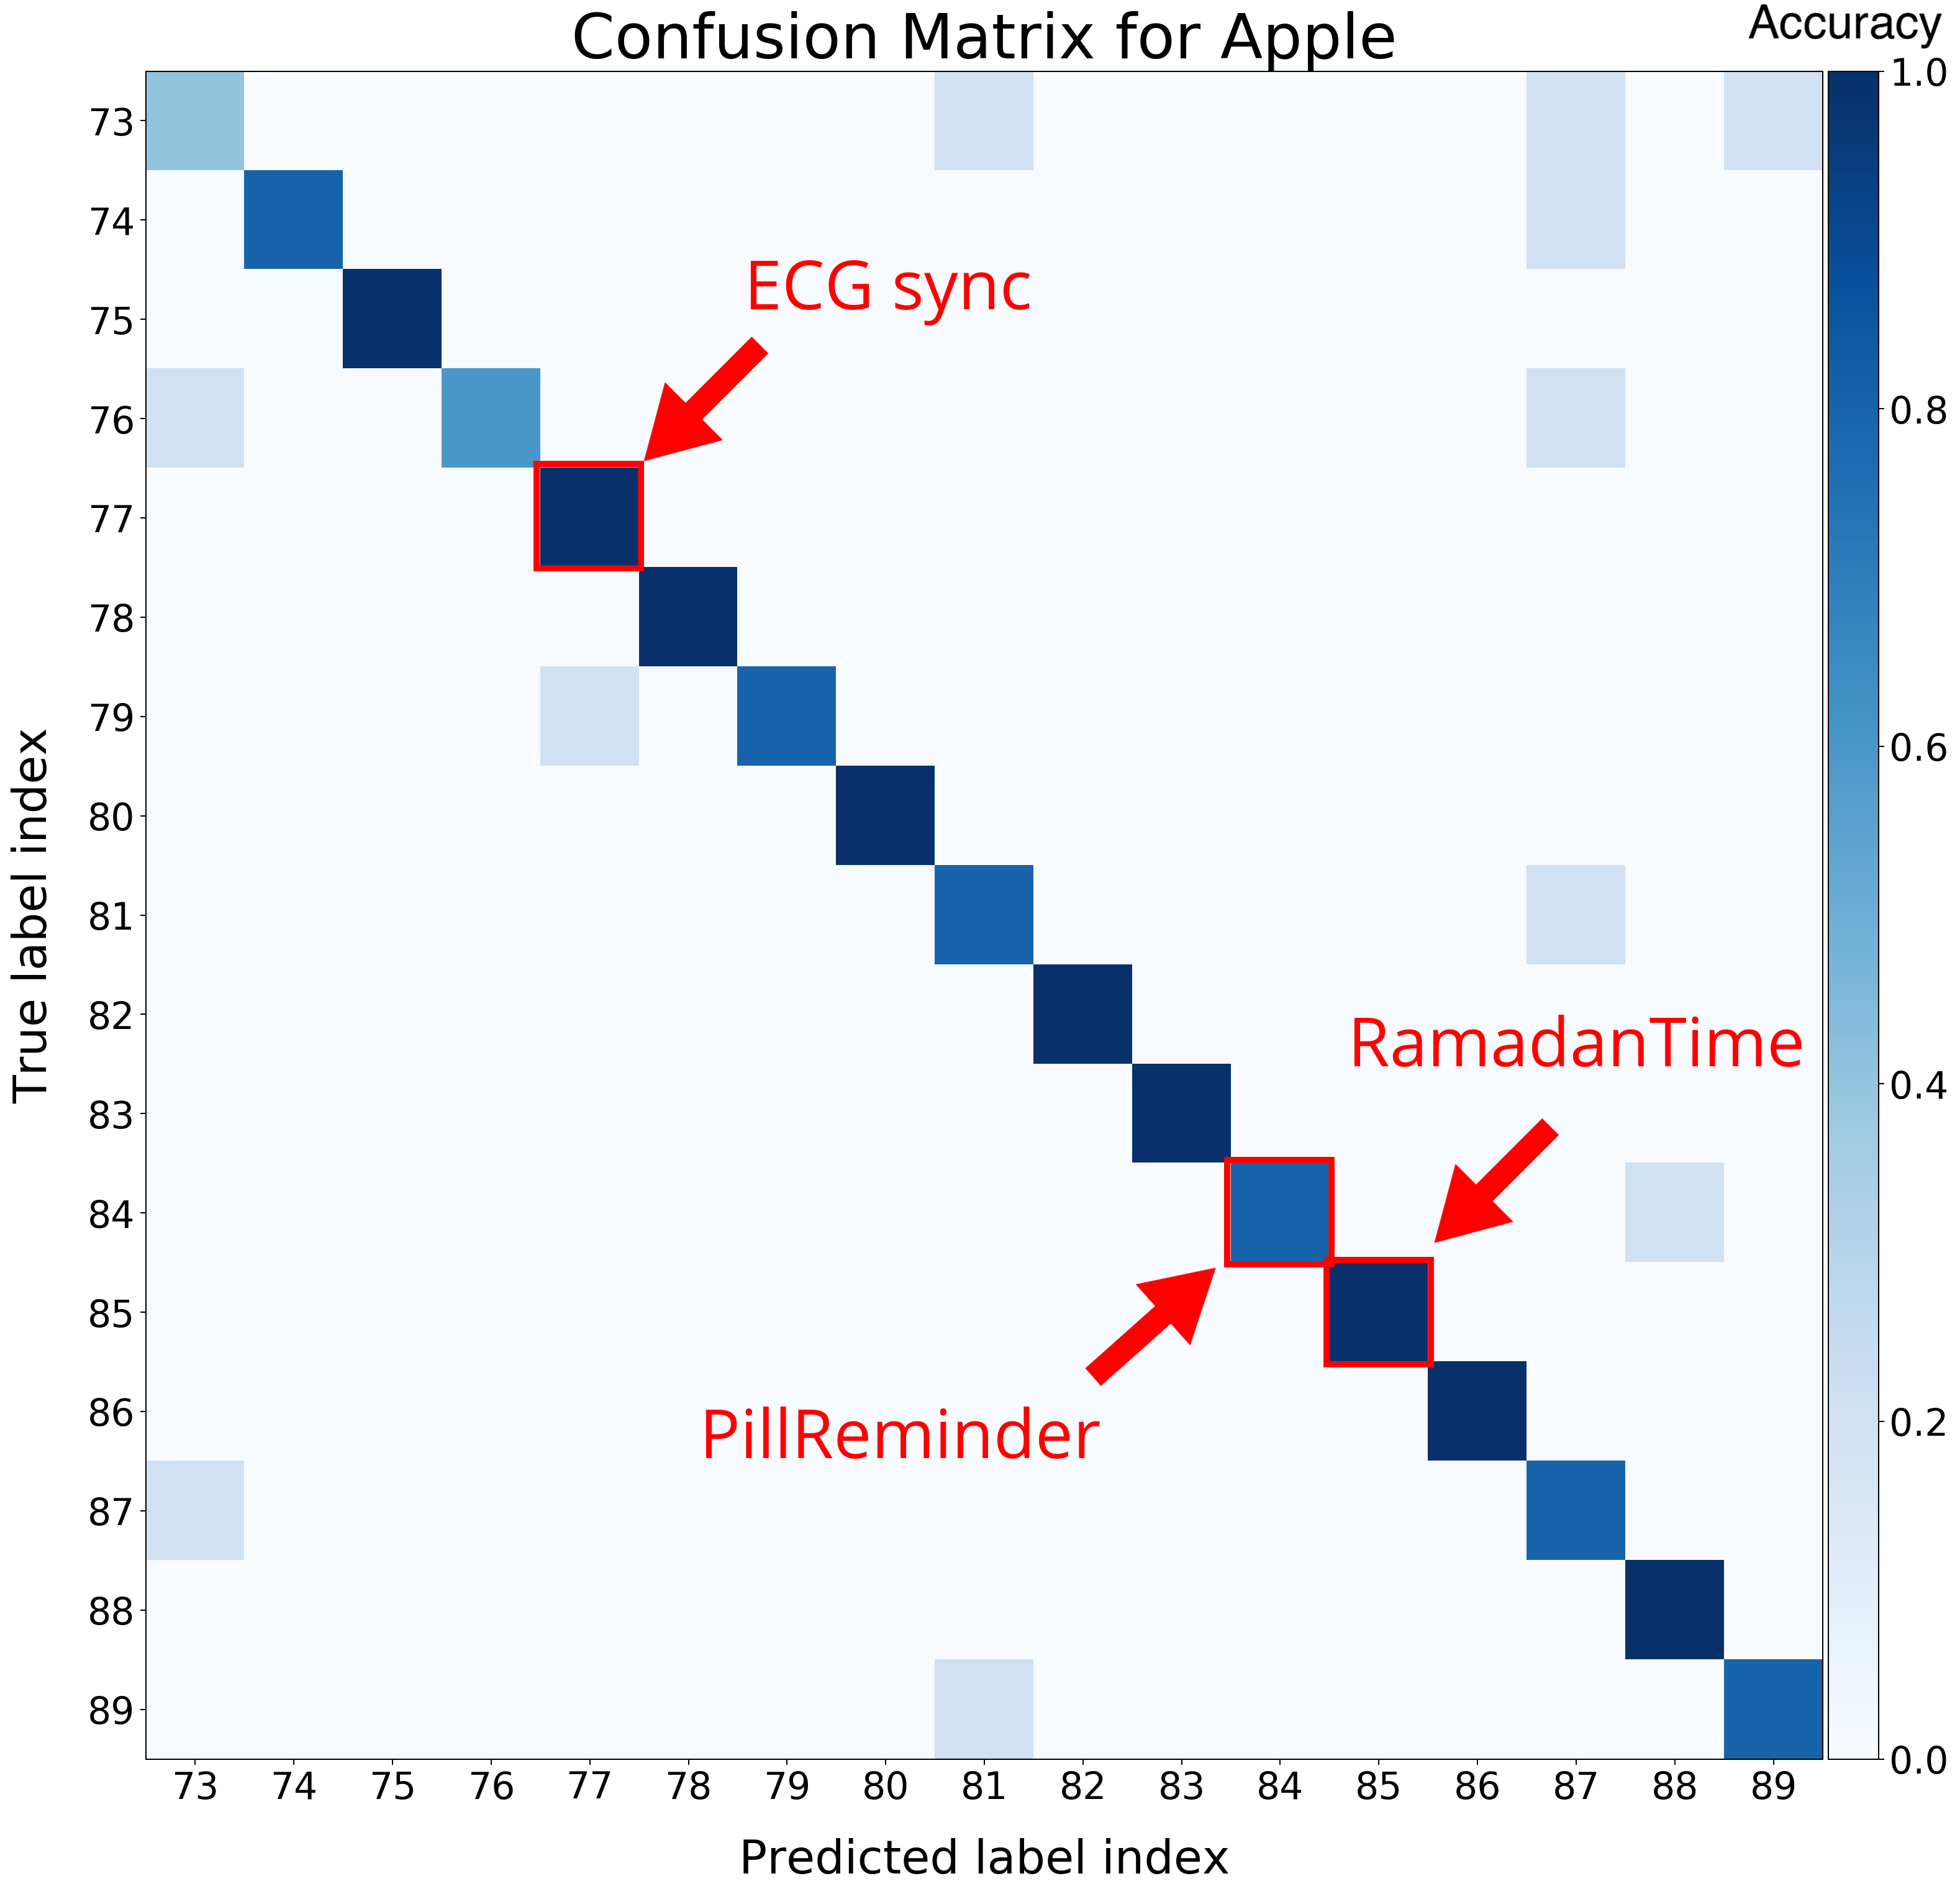
\includegraphics[width=0.7\textwidth]{figures/cm/Confusion_matrix_for_iwatch_annoted.png}
 \caption{Confusion matrix for Apple watch.}
 \label{fig:cm_iwatch}
\end{figure}






\section{Chapter Summary}
\label{chapter summary}
In this Chapter, we saw that encrypted Bluetooth traffic of smartwatches is highly subject to fingerprinting. Actions related to the same application might be hard to differentiate but are not likely to be confused with actions related to other applications. We also saw that the attack works on different devices. We give a summary of the results in Tab.~\ref{tab:results summury}. 
\\

\begin{table}[ht]
\centering

 \begin{tabular}{@{}llcccc@{}} 
 \toprule
  smartwatch-phone & actions targeted & accuracy & 95\% conf. & nb. class & nb. samples/class \\ [0.5ex] 
 \midrule
 Huawei-Pixel & opening  & 96.8\% &  2\% & 38 & 38\\ 

 Huawei-Pixel & in-app & 68.2\% & 7.1\% & 17 & 39\\
 
 Huawei-Pixel & opening \& in-app & 88.5\% & 2.6\% & 55 & 38\\

 Fossil-Nexus & opening & 90.5\% & 3\% & 35 & 28\\
 
 AppleWatch-iPhone & mix & 88.7\% &  7.5\% & 17 & 20  \\
 
 \bottomrule
 
\end{tabular}
%\caption{Sample of selected applications with short description and the criteria of selection}
 %   \label{tab:app_examples}

\caption{Results on the different experiments run in this Chapter.}
    \label{tab:results summury}
\end{table}


However, one question remains: How performs the attack on the whole set of actions on Huawei-Pixel? We explored opening and in-app actions but not both at the same time. Thus, we run the attack one more time on the set of all actions. This time, since the dataset is bigger, to ensure a good evaluation of the model, we used 200 random splits for cross-validation. The overall accuracy score is \textbf{88.5\% (+/- 2.6\%)}. The lowest F1 score of a targeted action is \textbf{30.78 (+/- 25.02)} whereas the best F1 score achieves \textbf{100\%}. We give samples of score achieved by different classes in Tab.~\ref{tab:rank summarize}.  We give an overall ranking and their associated score over the 55 actions in the Appendix (see Tab. \ref{tab:attack ranking}).
\\

\begin{table}[H]
\centering
 \begin{tabular}{llllll} 
 \toprule
 application name & action & F1 score & precision & recall \\ [0.5ex] 
 \midrule
FoursquareCityGuide & coffee & \textbf{30.78 (+/- 25.02)} & 32.96 (+/- 28.62) & 30.57 (+/- 28.12)\\
DiabetesM & addInsulin & 74.19 (+/- 18.89) & 73.85 (+/- 23.32) & 76.38 (+/- 26.60)\\
Shazam & open & 95.08 (+/- 9.28) & 99.17 (+/- 5.67) & 91.69 (+/- 16.07)\\
 Lifesum & addFood & 99.51 (+/- 3.78) & 99.13 (+/- 6.87) & 99.95 (+/- 1.41)\\
DiabetesM & open & \textbf{100.00 (+/- 0.00)} & 100.00 (+/- 0.00) & 100.00 (+/- 0.00)\\
 \bottomrule
\end{tabular}
\caption{Samples extracted from the overall ranking in Tab.~\ref{tab:attack ranking}. }
    \label{tab:rank summarize}
\end{table}